\section{Merkle Tree Library} \label{sec:merkle-tree-library}

As discussed in Section \ref{section:merkle-trees}, the integrity verification
protocol relies fundamentally on the Merkle tree data structure. Despite the widespread use of Merkle trees in the literature and in applications such as blockchains, there are relatively few general-purpose and reusable libraries available online. This is largely because implementations are often developed \textit{ad hoc}, tailored to the needs of a specific infrastructure or application domain.

To overcome this limitation, a dedicated library was developed in Rust\footnote{\url{https://www.rust-lang.org}}, named \texttt{mt-rs}. The library is distributed under a BSD-3 Licence on Crates.io\footnote{\url{https://crates.io/crates/mt-rs}}, with its source code publicly available at \url{https://github.com/boozec/mt}.

\paragraph{Hasher}

The construction of a Merkle tree begins with the definition of a \textit{hasher}, i.e., the cryptographic hash function applied to the leaves and internal nodes of the tree. This enables direct experimentation with different trade-offs between performance and security. The design allows developers to implement custom hashers by instantiating the trait \texttt{Hasher}, which requires only the implementation of the \texttt{hash} method. Listing \ref{code:hasher-example} illustrates a simple example of a user-defined hasher.


\begin{listing}[!ht]
\caption{Example of a custom hasher \texttt{FooHasher}, which hashes an input as a string with the prefix "foo\_" followed by the sum of the integer values of its bytes, in hexadecimal format.}
\label{code:hasher-example}
\begin{minted}[linenos,fontsize=\footnotesize]{Rust}
use mt_rs::hasher::Hasher;

pub struct FooHasher;

impl Hasher for FooHasher {
    fn hash(&self, input: &[u8]) -> String {
        let sum: u32 = input.iter().map(|&b| b as u32).sum();
        format!("foo_{:x}", sum)
    }
}
\end{minted}
\end{listing}


The library provides three default hashers: \texttt{SHA256Hasher}, \texttt{Keccak256Hasher}, and \texttt{Blake3Hasher}. They correspond to the functions analyzed in Section \ref{sec:cryptopgrahic-hash-functions}. 

\paragraph{Tree construction}
A Merkle tree is represented by the structure shown in Listing \ref{code:struct_merkletree}. It can be instantiated either from raw in-memory data using the \texttt{new} method or from the contents of files and folders using the \texttt{from\_paths} method (Listing \ref{code:new_and_from_paths_prototypes}). This dual approach supports both synthetic testing and real-world scenarios, such as integrity verification of storage systems, by avoiding repeated disk reads.

\begin{listing}[!ht]
\caption{\texttt{MerkleTree} structure definition, where \texttt{Node} is an ad hoc structure that includes additional information and methods.}
\label{code:struct_merkletree}
\begin{minted}[linenos,fontsize=\footnotesize]{Rust}
pub struct MerkleTree {
    /// Leaf nodes at the base of the tree 
    /// (may include a duplicate for even pairing).
    leaves: Vec<Node>,
    /// Height of the tree (number of levels including root).
    height: usize,
    /// Root node of the Merkle tree.
    root: Node,
}
\end{minted}
\end{listing}


\begin{listing}[H]
\caption{Signatures of the \texttt{new} and \texttt{from\_paths} methods. A concrete \texttt{Hasher} is always provided when defining a Merkle tree.}
\label{code:new_and_from_paths_prototypes}
\begin{minted}[linenos,fontsize=\footnotesize]{Rust}
impl MerkleTree {
    pub fn new<I, T, H>(hasher: H, data: I) -> Self
    where
        I: IntoIterator<Item = T>,
        T: AsRef<[u8]>,
        H: Hasher + 'static + std::marker::Sync,
    { /* ... */ }

    pub fn from_paths<H>(hasher: H, paths: Vec<String>) -> Self
    where
        H: Hasher + 'static + std::marker::Sync + Clone,
    { /* ... */ }
}
\end{minted}
\end{listing}

Internally, both methods translate the input data into leaf nodes of type \texttt{Node} and then invoke the builder function (Listing \ref{code:mt-build}), which assembles the tree level by level. The construction algorithm ensures binary balance by duplicating the last node when the number of nodes is odd.

Parallelization is achieved through the \texttt{par\_chunks} method of the Rayon crate\footnote{\url{https://crates.io/crates/rayon}}, which splits slices into disjoint chunks and computes parent nodes concurrently.

The tree is organized into \emph{levels}: the leaves at Level 1, the root at the highest level, and internal nodes in between (Figure \ref{fig:merkle-tree-levels}). This layered representation makes the structure conceptually simple. The root node is accessible through the \texttt{root()} method, and its hash can be retrieved directly. Unlike leaves and the root, internal nodes are not stored explicitly in the \texttt{MerkleTree} structure.

\begin{figure}[!ht]
\centering
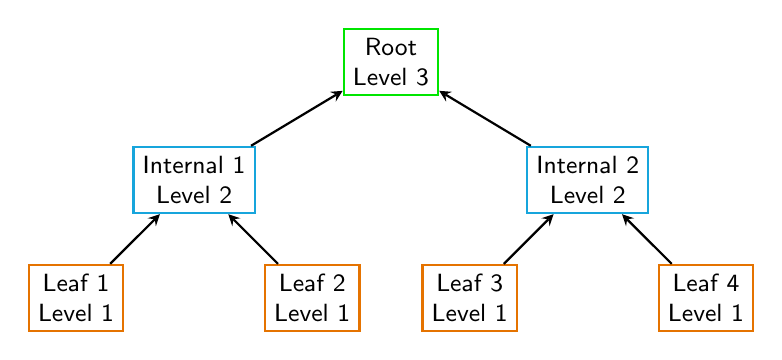
\begin{tikzpicture}[
  every node/.style={font=\sffamily\small, draw, rectangle, minimum size=8mm, align=center},
  greenborder/.style={draw=green!90!black, thick},
  blueborder/.style={draw=cyan!90!black, thick},
  yellowborder/.style={draw=orange!90!black, thick},
  level 1/.style={sibling distance=50mm, level distance=15mm},
  level 2/.style={sibling distance=30mm, level distance=15mm},
  level 3/.style={sibling distance=15mm, level distance=15mm},
  edge from parent/.style={draw, thick, <-, >=stealth}
]

% Root
\node[greenborder] {Root\\Level 3}
  child {node[blueborder] {Internal 1\\Level 2}
    child {node[yellowborder] {Leaf 1\\Level 1}}
    child {node[yellowborder] {Leaf 2\\Level 1}}
  }
  child {node[blueborder] {Internal 2\\Level 2}
    child {node[yellowborder] {Leaf 3\\Level 1}}
    child {node[yellowborder] {Leaf 4\\Level 1}}
  };

\end{tikzpicture}
\caption{An example of a binary Merkle tree with 4 leaves, showing the different levels: leaves (Level 1), internal nodes (Level 2), and the root (Level 3).}
\label{fig:merkle-tree-levels}
\end{figure}

\begin{listing}[H]
\caption{Build method for constructing the Merkle tree from the leaves upward. The \texttt{height} variable tracks the number of levels.}
\label{code:mt-build}
\begin{minted}[linenos,fontsize=\footnotesize]{Rust}
impl MerkleTree {
    fn build<H>(hasher: H, mut leaves: Vec<Node>) -> Self
    where
        H: Hasher + 'static + std::marker::Sync,
    {
        let original_leaves = leaves.clone();
        let mut height = 1;

        while leaves.len() > 1 {
            if leaves.len() % 2 != 0 {
                leaves.push(leaves.last().unwrap().clone());
            }

            leaves = leaves
                .par_chunks(2)
                .map(|pair| {
                    let combined = [
                        pair[0].hash().as_bytes(),
                        pair[1].hash().as_bytes()
                    ]
                    .concat();
                    
                    let hash = hasher.hash(&combined);
                    
                    Node::new_internal(hash, pair[0].clone(), pair[1].clone())
                })
                .collect();

            height += 1;
        }

        MerkleTree {
            leaves: original_leaves,
            height,
            root: leaves.into_iter().next().expect("root not found"),
        }
    }

}
\end{minted}
\end{listing}

Listing \ref{code:mt-root-print} demonstrates printing the Merkle tree root hash. The \texttt{hash()} method of each node returns the computed hash as a string.
\begin{listing}[H]
\caption{Snippet of code that prints the Merkle root hash of a tree with two byte strings as leaves.}
\label{code:mt-root-print}
\begin{minted}[linenos,fontsize=\footnotesize]{Rust}
let data = &["hello".as_bytes(), "world".as_bytes()];
let tree = MerkleTree::new(Blake3Hasher::new(), data);
println!("Merkle root: {}", tree.root().hash());
\end{minted}
\end{listing}

\paragraph{Proof generation and verification}
The library also supports Merkle proofs, which enable verification that a given leaf belongs to a specific Merkle tree. Proofs are generated and verified via implementations of the \texttt{Proofer} trait (Listing \ref{code:mt-proofer-trait}). A Merkle proof is expressed as sequences of \texttt{ProofNode} elements, which encode the sibling hashes encountered on the path from the leaf to the root. Users may define custom proofers if needed.

\begin{listing}[!htb]
\caption{The \texttt{Proofer} trait.}
\label{code:mt-proofer-trait}
\begin{minted}[linenos,fontsize=\footnotesize]{Rust}
/// Represents a single step in a Merkle proof path.
pub struct ProofNode {
    pub hash: String,
    pub child_type: NodeChildType, // Left or Right
}

/// A Merkle proof containing the path from a leaf to the root.
pub struct MerkleProof {
    pub path: Vec<ProofNode>,
    pub leaf_index: usize,
}

pub trait Proofer {
    /// Generates a Merkle proof for the data at the specified index
    fn generate(&self, index: usize) -> Option<MerkleProof>;

    /// Verifies that a piece of data exists in the tree using a Merkle proof
    fn verify<T>(&self, proof: &MerkleProof, data: T, root_hash: &str) -> bool
    where
        T: AsRef<[u8]>;
}
\end{minted}
\end{listing}


In this work, the \texttt{DefaultProofer} is used. Its implementation corresponds to proof generation (Algorithm \ref{algo:merkle-proof-generation}) and proof verification (Algorithm \ref{algo:merkle-proof-verification}). Unlike the \texttt{MerkleTree} structure, which does not store internal nodes, the \texttt{DefaultProofer} retains all levels.


Verification proceeds by iteratively reconstructing the root hash from the leaf and its authentication path, comparing the result with the expected root. The implementation in Rust is reported in Listing \ref{code:default-proofer}.

\begin{listing}[!htp]
\caption{Implementation of the \texttt{Proofer} trait for \texttt{DefaultProofer}. The proof is built by traversing the tree levels and collecting sibling hashes along the path.}
\label{code:default-proofer}
\begin{minted}[linenos,fontsize=\footnotesize]{Rust}
impl<H> Proofer for DefaultProofer<H>
where
    H: Hasher,
{
    fn generate(&self, index: usize) -> Option<MerkleProof> {
        if index >= self.levels[0].len() { return None; }
        let mut path = Vec::new();
        let mut current_index = index;
        for level in &self.levels[..self.levels.len() - 1] {
            let sibling_index = (current_index ^ 1).min(level.len() - 1);
            let sibling = &level[sibling_index];
            let child_type = if sibling_index < current_index {
                NodeChildType::Left
            } else {
                NodeChildType::Right
            };
            path.push(ProofNode {
                hash: sibling.hash().to_string(), child_type 
            });
            current_index >>= 1;
        }
        Some(MerkleProof { path, leaf_index: index })
    }

    fn verify<T>(&self, proof: &MerkleProof, data: T, root_hash: &str) -> bool
    where
        T: AsRef<[u8]>,
    {
        let mut current_hash = self.hasher.hash(data.as_ref());
        for proof_node in &proof.path {
            let combined: String = match proof_node.child_type {
                NodeChildType::Left => 
                    format!("{}{}", proof_node.hash, current_hash),
                NodeChildType::Right => 
                    format!("{}{}", current_hash, proof_node.hash),
            };
            current_hash = self.hasher.hash(combined.as_bytes());
        }
        current_hash == root_hash
    }
}
\end{minted}
\end{listing}

\newpage

\paragraph{Example and Conclusion}  
The complete workflow of the library is illustrated in Listing~\ref{code:mt-example}.
In this test, a Merkle tree is constructed from the folder \emph{pics}, which contains three files. The program verifies the basic properties of the tree, such as its height, and root hash, before generating a Merkle proof for the first leaf.  
Finally, the proof is successfully verified against the computed root hash, confirming the correctness of both tree construction and proofing. This example brings together the key components of the \texttt{mt-rs} library (hashers, tree building, and proof generation) and demonstrates their integration in practice, concluding the presentation of the Merkle tree library by showing how the system operates end-to-end on real data.


\begin{listing}[!htb]
\caption{End-to-end test of the \texttt{mt-rs} library: building a Merkle tree from the folder \emph{pics} (with three files), checking its properties, and verifying that a proof for the first leaf matches the expected root hash.}

\label{code:mt-example}
\begin{minted}[linenos,fontsize=\footnotesize]{Rust}
let hasher = Blake3Hasher::new();
let folders = vec![String::from("pics/")];

let tree = 
    MerkleTree::from_paths(hasher.clone(), folders);

assert_eq!(tree.height(), 3);
assert_eq!(
    tree.root().hash(),
    "a08c44656fb3f561619b8747a0d1dabe97126d9ed6e0cafbd7ce08ebe12d55ca"
);

let proofer = DefaultProofer::new(
    hasher.clone(), 
    // Recursively hashes the contents of files and directories.
    hash_dir(hasher.clone(), folders), 
);

let proof = proofer.generate(0).expect("proof generation failed");

assert!(proofer.verify(
    &proof,
    // Read the content of the first leaf read by the folder pics/
    &fs::read("pics/photo0.png").expect("file not found"),
    "a08c44656fb3f561619b8747a0d1dabe97126d9ed6e0cafbd7ce08ebe12d55ca"
));
\end{minted}
\end{listing}
